In order to obtain a mission specification and a robot plan compatible with the open world assumption, we need to address two main problems. First of all, the specification itself has to allow for self-updates during execution. Second, the specification has to be automatically re-written, in order to incorporate the newly discovered elements of the open world, such as new mission objectives. Finally, re-synthesis will take place, in order for the changes to be reflected in the robot's discrete strategy.

We begin by giving a broad definition of \emph{open world}, specific to the current context; that of controller synthesis.

\begin{myDefinition}\label{Def:openworld}
	\textbf{(Open World):} . We say that the robot operates in an open world if the state-space $\SSS$ grows during execution. Specifically, we define the open world function $$\mathcal{W}(\SSS, \mathit{x}, \mathit{y}) = \hat{\SSS} = \hat{\mathcal{X}} \cup \hat{\mathcal{Y}},$$
	where $\hat{\mathcal{X}} = \mathcal{X} \cup \left\{ \mathit{x} \right\}$, $\hat{\mathcal{Y}} = \mathcal{Y} \cup \left\{ \mathit{y} \right\}$, and $\mathit{x}, \mathit{y} \neq \emptyset \Rightarrow \mathit{x}, \mathit{y} \not \in \SSS $.
	\end{myDefinition} 
% TODO: define open world function?
The elements $\mathit{x}, \mathit{y}$ are possible new environment and robot propositions, respectively. We will return to this definition in Section \ref{openworld}, where we add additional structure and make use of a more narrow domain of the open world function $\mathcal{W}$.

Given the definition above, there are two three reasons that motivate the need for open world mission specifications. First of all, in real-world applications, such as autonomous search and rescue scenarios, the mission is often specified before the robot has obtained full knowledge of the world. Second, the robot may have to incorporate new function and components to its strategy. Finally, the state-space may be too large for the user to enumerate every possible variation a priori (see Example \ref{Ex:mailbot1} below).  To clarify these reasons, we introduce an illustrative example:

\begin{myExample}\label{Ex:mailbot1} Autonomous Mailbot (Fig. \ref{Fig:pr3})\\
	A robotic courier (mailbot) operates within a school or company building. It is tasked with collecting letters and delivering them to the recipients' offices. Even if all possible recipients and the locations of their offices are fixed, the information may not be available at the time the mission specification is defined. 
\end{myExample}

\begin{figure}[ht]
	\centering
	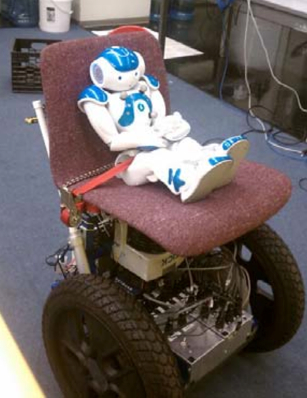
\includegraphics[width=0.7\columnwidth, clip]{./img/pr3.jpg}
	\caption{Our implementation of a mailbot. A Nao humanoid robot (ref ???) is mounted on a segway platform. The actuation and perception capabilities of the former are complemented by the localization, navigation and mobility advantages of the latter.}
	\label{Fig:pr3}
\end{figure}

In the example above, notice that the robot does not operate serially, i.e., collecting one letter, delivering it, and returning for the next one. Rather, it is allowed to carry multiple letters at once, collect letters on its way to delivering a different letter, etc. Therefore, the specification must make sure that the robot only delivers letters at the correct location, that it is aware of which letters it is carrying, and that it does not forget to deliver a letter altogether. The open world aspect of the mission comes from the fact that new letters that correspond to new recipients may be collected by the robot. Therefore, it is not possible to explicitly write a specification in the form of individual tasks, e.g., \texttt{if you are sensing letter\_John\_Doe then do PickUp and go to John\_Does\_office}.

Given the ``symmetry" of the individual delivery tasks of Example \ref{Ex:mailbot1} (bring letters to offices), the ability to describe the robot's mission in more abstract terms would be desirable. In general, operation in an open world will result in new region, action, and environment propositions, as well as additional mission goals, all of which have to be (i) taken into account \emph{implicitly} in the initial mission specification, and (ii) incorporated in the specification on-the-fly.

The first problem we aim to solve is a practical one. In a scenario such as that of Example \ref{Ex:mailbot1}, parts of the robot's state space (e.g. letters to carry) are potentially very large and could conceivably be expanded (or reduced) by the user in subsequent runs. To specify the same reactive behavior over an additional proposition in the domain, the user would have to modify or duplicate nearly every sentence in the specification. A more preferable approach would be to specify behaviors with an abstraction that does not explicitly refer to individual propositions.

\begin{myProblem}\label{Prop:groups}
	\textbf{(Specification Abstractions):}
	Given a robot mission that includes indentical behavior over multiple propositions, express that mission in a specification language such that the individual propositions acted on identically are not explicitly referred to. 
\end{myProblem}

Our approach to Problem 1 is to include elements of first-order logic in our specification language, specifically set operations. We will first explain the theory and use of these abstractions in our specifications (Section \ref{abstractions}), and then apply them to the second part of our overall problem, updating an open world mission specification (Section \ref{openworld}). 

% END